%0       1         2         3         4         5         6         7         8
%2345678901234567890123456789012345678901234567890123456789012345678901234567890
%
%
%
% \section{Petascale Astrophysics Review}
%   \subsection{\enzo}
%   \subsection{FLASH}
%   \subsection{CHOMBO}
%   \subsection{GADGET-2}
% 
% \section{Cello}
% \subsection{Science Goals}
% \subsection{Software Goals}
% \subsubsection{Adaptive Mesh Refinement}
% \subsubsection{Particles}
% \subsubsection{Hyperbolic and Elliptic Methods}
% \subsubsection{Dynamic Task Scheduling}
%    CHARM++
%
% OUTLINE
% SUMMARY
% EXTREME SCALING ISSUES
%    Hardware-related issues
%    Data structure scaling issues
% REVIEW
%    Paramesh
%    CHOMBO
%    SAMARAI
% CELLO 
%    particle precision
%    grid position
%    timestepping
% REQUIREMENTS: scope of library / framework
%    capabilities
%       physics
%          hyperbolic
%          elliptic
%          ray-tracing?
%       AMR
%       Particles
%       performance
%       parallel scaling
%       data structure scaling
%       ease of use
%       dynamic scheduling
%       aggressive minimization of global communication
%       I/O
%       fault tolerance
%       adaptivity
%       extensibility
% DESIGN: software organization and data structures
%    high-level design
%       OOP
%       components
%          Simulation, Control, Parallel, Task
%          Amr, Patch: stores the AMR hierarchy
%          Fields, Particles, Array: for storing data
%          Block, Fluxes: for computing / communicating data
%          Performance, Error, Parameters, Memory
%             globally-accesible functions; components in
%             aspect-oriented programming paradigm; not sufficiently
%             important to use AspectC, but techniques (primarily
%             using templates) usable
%          Method [Analysis] [Visualize]
%             hooks to user code; multiple methods permitted,
%             selectable and scheduled at run-time
%       user interface
%          External, User
%       application-driven
%    data structures
%
% ALGORITHMS: and how problems solved
%    AMR
%    particles
%    parallelization
%    load balancing
%    fault tolerance
% IMPLEMENTATION
%    Languages: C++, C99, UPC, OpenMP
%    Libraries: HDF5, MPI
%    Frameworks: CHARM++, OpenCL
%    TRAC
%      wiki used for design
%      tickets for tasks and documenting defects
%    Subversion
%    unit testing
%    regression testing
%      lcatest
%      correctness, single-thread performance, weak and strong parallel scaling
%          shallow and deep problems
%      lcaperf
%    software reviews

% Requirements
%    
% Design
% Implementation




%=======================================================================
\documentclass{article}
%=======================================================================


% INCLUDE DEVELOPMENT TEXT

\newcommand{\devel}[1]{\textbf{#1}}

% EXCLUDE DEVELOPMENT TEXT

% \newcommand{\devel}[1]{}


%=======================================================================
% Document layout
%=======================================================================

\setlength{\topmargin}{0.0in}
\setlength{\oddsidemargin}{0.0in}
\setlength{\evensidemargin}{0.0in}
\setlength{\textwidth}{6.0in}
\setlength{\textheight}{9.0in}

%=======================================================================
% Packages
%=======================================================================

\usepackage{wasysym}
\usepackage{epsfig}
\usepackage{url}

%=======================================================================
% Commands
%=======================================================================

\newcommand{\cello}{\textsf{Cello}}
\newcommand{\enzo}{\textsf{Enzo}}
\newcommand{\lcaperf}{\textsf{lcaperf}}
\newcommand{\lcatest}{\textsf{lcatest}}

\newcommand{\code}[1]{\textsf{#1}}

\newcommand{\note}[1]{\devel{\eighthnote\ \textit{#1} \\}}
\newcommand{\pargraph}[1]{\devel{\P\ \textbf{#1} \\}}

\newcommand{\todo}{\devel{$\circ$}}
\newcommand{\done}{\devel{$\bullet$}}
\newcommand{\halfdone}{\devel{\textcolor{gray}{$\bullet$}}}

\newcommand{\PROJECT}{\cello}

\newcommand{\TITLE}[3]{
\title{ {\huge \PROJECT\ #1}  \\ \vspace{0.1in}
     {\small Document Version: \textbf{#3}} \vspace{-0.1in}
    }
\author{      #2 \\
        Laboratory for Computational Astrophysics\\
        University of California, San Diego}
\maketitle}

%=======================================================================


\usepackage{natbib}

%=======================================================================

\begin{document}

\nocite{StSh09} % Scalability challenges for massively parallel {AMR} applications
\nocite{WiHy03} % Enhancing scalability of parallel structured {AMR} calculations
\nocite{GuWi06} % Parallel clustering algorithms for structured {AMR}
\nocite{BuGh08} % Towards adaptive mesh {PDE} simulations on petascale computers

%=======================================================================
\TITLE{A Software Framework for Extreme Adaptive Mesh Refinement}{James Bordner}{$Rev$}
%=======================================================================

% \renewcommand{\pargraph}[1]{}

%=======================================================================
\section{Project Summary} \label{s:summary}
%=======================================================================

%
\pargraph{Motivation}
%
\pargraph{Proposal}
We propose to develop a new software library for adaptive mesh
refinement (AMR) that allows application developers to develop
multiphysics applications for simulating phenomena on an extreme range
of spacial and temporal scales, and that require an extreme amount of
computation, memory, and storage (petascale and exascale).
%
\pargraph{data structure scope summary}
Our basic data structure is a fully parallel distributed octree, with
associated array and particle data, thus supporting both Eularian, Lagrangian,
and hybrid methods such as Particle Mesh (PM).
%
\pargraph{parallelization strategy}
Multiple parallelization technologies can be used, including hybrid
approaches such as MPI or UPC for distributed memory data, and UPC or
OpenMP for shared memory data.  CHARM++ will also be supported.
Extreme scalability will be obtained by localizing the patch / block
problems as much as is feasible; this will help control scalability
issues related to limited floating-point precision and ranges, as well
as reducing the need for global synchronization and reduction
operations.
%
\pargraph{load balancing}
Dynamic load balancing will be hierarchical, both to better adapt to
the hierarchical nature of extreme scale computational platforms, and
to allow flexibility in load balancing frequency and metrics at different
levels.
%
\pargraph{fault tolerance}
Fault tolerance and software resilience are crucial factors at extreme scales,
since it has been observed that frequency of failures is proportional to
the number of sockets.
due to the reduced MTTI (mean time to interrupt) , since the probability that hardware component, operating system, library, or application component fails Unfortunately, approaches to fault tolerance are still 
%
\pargraph{I/O}
Disk I/O is also a crucial factor for petascale 

\pargraph{availablity}
We plan to make this framework publicly available for scientific research use.

Advantage: designing with extreme scale in mind from the beginning.

DOE buzzwords
\url{http://www.er.doe.gov/ASCR/WorkshopsConferences/MathTalks/M\_wright.pdf}

AMR \\
applied mathematics\\
collaborative software environments\\
computer science technologies\\
exascale \\
extreme scale\\
failure avoidance \\
failure effects avoidance \\
fault tolerance\\
GPU \\
HPC \\
memory hierarchy\\
multicore\\
multiphysics \\
multiscale \\
one-sided communication\\
performance tuning\\
petascale \\
PGAS \\
research goals\\
resilient software \\
UPC \\
virtual processes \\

\note{describe existing  technology: Flash, Chombo}
\note{describe contributions: improved tree-based AMR}
\note{distributed datastructure}
\note{multilevel parallelism}
\note{dynamic execution and communication scheduling: prefetch messages}
\note{dependencies known: patch can advance when its neighbor data is known}

\url{http://diversity.doe.gov/documents/Writing\_Winning\_Proposals.pdf}

milestones

decision points

justify course of action

highlight innovative features

leverage collaborators

get RFP

get sample proposals

get evaluation factors list

preliminary results

good references critical; only give great references

use rfp keywoards

quality control

sustainability--what happens when money ends

deliverables: software, research papers, workshop/training

sales document not technical manual


%=======================================================================
\section{Extreme Scaling Issues} \label{s:scaling}
%=======================================================================

Petascale AMR research issue.


\pargraph{equation scope}
Nonlinear time-dependent hyperbolic conservation laws, and elliptic PDE's

\begin{itemize}
\item synchronization and collective operations
\item parallel I/O
\item fault tolerance / software resiliency
\item distributed data structures
\item hierarchical memory
\item hierarchy parallelism
\item dynamic load balancing
\item heterogeneous computational components: GPU's
\item ease of use: unigrid update + interpolation + flux correction
\item weigh advantages / disadvantages of patch- versus tree-amr
\end{itemize}


\section{Review of Existing AMR frameworks}

\pargraph{CHOMBO}

  Block-structured AMR

\pargraph{SAMRAI}

   [2001]
   good scaling for numerical and data communication
   poorer scaling in adaptive meshing and communication schedule construction 

\pargraph{Paramesh}

  Octree-based AMR

GADGET-2: Preeminent cosmological TreeSPH simulation code
DAGH (1998)

\section{Project requirements}

\section{Project design}

General goals

\begin{itemize}
\item extreme parallel scalability
\item extreme data structure scalability
  \begin{itemize}
  \item breadth: number of grid patches
  \item depth: number of AMR hierarchy levels
  \end{itemize}
\end{itemize}

\begin{itemize}
\item for parallel scalability: aggressive minimization of
  synchronization and collective operations
\item ``localize'' problem as much as possible
  \begin{itemize}
  \item For each patch, only store patch, location information for
    neighboring patches (``ghost patches''), and ancestors for octree
  \item patch-local adaptive timestep control
    \begin{itemize}
    \item prevents rapidly evolving feature in one localized region of
      domain from determining timestep elsewhere
    \end{itemize}
  \end{itemize}
\item facilitate dynamic load balancing, dynamic scheduling of
  communication and computation
\item maximize data structure flexibility
\item dynamically optimize data structure parameters to hardware
  during run time
\item for algorithmic scalability: aggresively minimize dependencies
  of fp and integer precision on data structure size
\item related to ``localization'' of tasks
  \begin{itemize}
  \item particle positions stored using local coordinate system with
    origin at patch corner
  \item absolute patch coordinates not stored, only position relative
    to neighbors
     \begin{itemize}
     \item global coordinates only needed for initialization
     \item only need mesh width and timestep size for advancing
     \item not needed for restarts
     \item can still be computed dynamically
     \item localization an option--not needed for smaller problems
     \item absolute particle positions / grid locations may be needed
       for some output, e.g. global particle analysis
     \item in that case low precision
     \item still scaling issues relative to depth
      \begin{itemize}
      \item neighbor location
      \end{itemize}
     \end{itemize}
  \end{itemize}
\end{itemize}

\begin{itemize}
\item targeted refinement by 4 or 8
  \begin{itemize}
  \item especially effective for deep AMR, e.g. star formation with
    30+ levels
  \item still supports effective resolution jumps of 2 using backfill
  \end{itemize}
\item patch coalescing
  \begin{itemize}
  \item reduced AMR overhead (number of patches) especially in shallow
    AMR relative to Paramesh
  \item improved performance since locally unifrom grid instead of AMR
    patches
  \item still supports variable block sizes for optimizing memory
    hierarchy, parallel task size, task counts
  \end{itemize}
\item variable patch resolution
\item instead of uniformly refining a patch, can replace with higher
  resolution array
\item need AMR machinery where resolution requirements change, not
  where high resolution is needed
\end{itemize}


\section{Project data structures and algorithms}

Amr, Tree, Array, Patch

\begin{center}
\begin{minipage}{7.0in}
\begin{minipage}{2.2in}
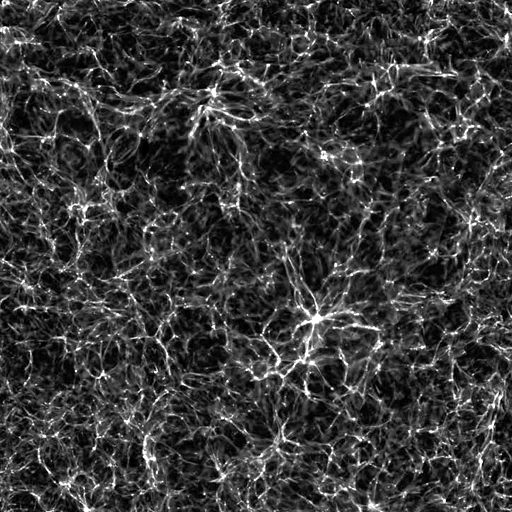
\includegraphics[width=2.2in]{cosmo2.png}
\end{minipage} \ 
\begin{minipage}{2.2in}
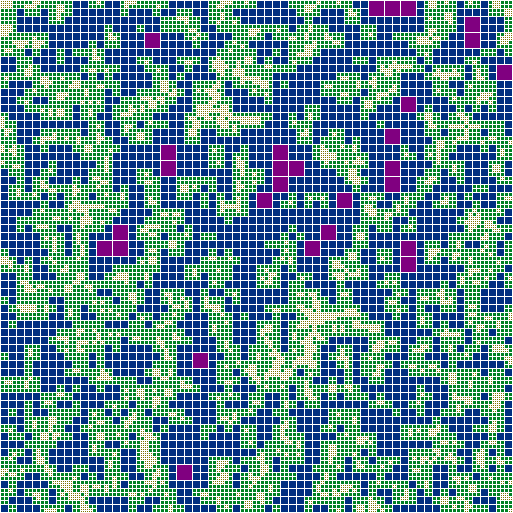
\includegraphics[width=2.2in]{cosmo2-4-1.png}
\end{minipage} \ 
\begin{minipage}{2.2in}
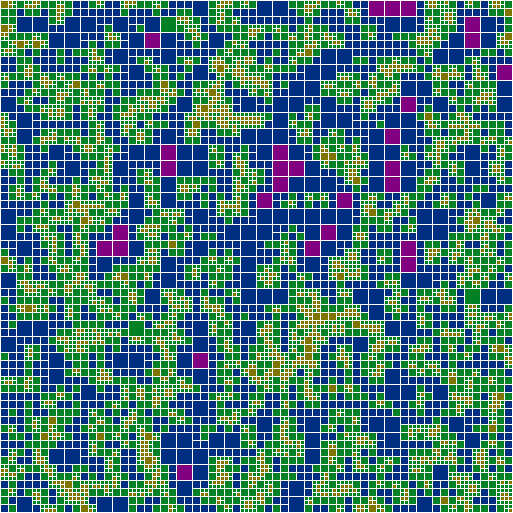
\includegraphics[width=2.2in]{cosmo2-4-2.png}
\end{minipage}
\end{minipage} \\
\ \\
\begin{minipage}{7in}
\textbf{Left}: 2D Source cosmology density field projection.  
\textbf{Middle}: Balanced octree: 81701 patches.
\textbf{Right}: Balanced octree with coalesced patches: 32529 patches.
\ \\
\end{minipage}
\end{center}


\begin{center}
\begin{minipage}{7.0in}
\begin{minipage}{2.2in}
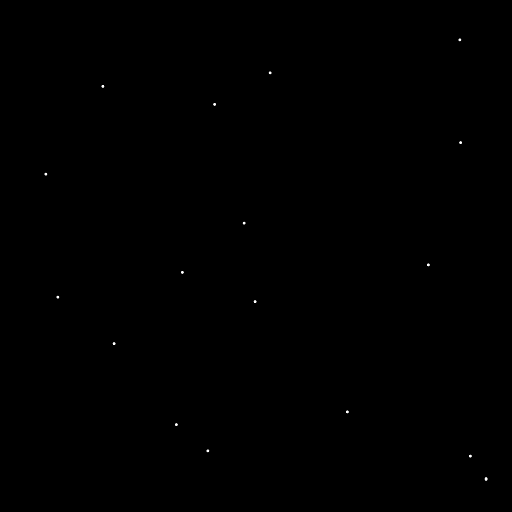
\includegraphics[width=2.2in]{dots.png}
\end{minipage} \ 
\begin{minipage}{2.2in}
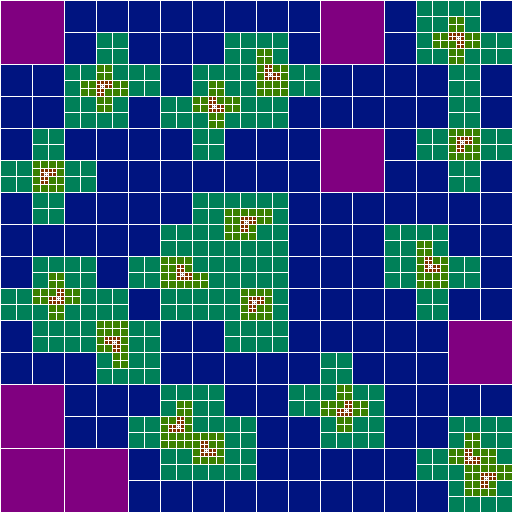
\includegraphics[width=2.2in]{dots-4-1.png}
\end{minipage} \ 
\begin{minipage}{2.2in}
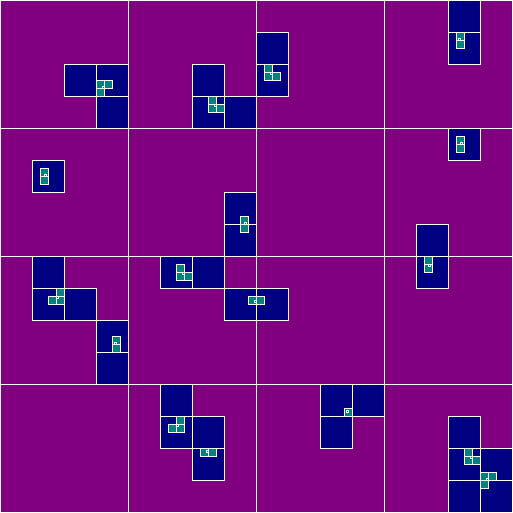
\includegraphics[width=2.2in]{dots-16-5.png}
\end{minipage}
\end{minipage} \\
\begin{minipage}{7in}
\begin{minipage}[t]{2.2in}
2D Source cosmology density field projection
\end{minipage} \ 
\begin{minipage}[t]{2.2in}
Balanced octree: 2137 patches
\end{minipage} \ 
\begin{minipage}[t]{2.2in}
Balanced sparse $4^3$-tree: 158 explicit patches
\end{minipage}
\end{minipage}
\end{center}

\begin{itemize}
\item generalized octree-based AMR 
  \begin{itemize}
  \item 8-tree, sparse 64-tree, sparse 512-tree
  \item decoupled AMR / Array
  \item 
  \end{itemize}
\item Fully distributed AMR data structure
  \begin{itemize}
\item For each local grid patch, only immediate neighbors and
  ancestors stored
  \item Proxies for remotely stored patches
    \begin{itemize}
    \item remote thread identifier + pointer
    \end{itemize}
  \end{itemize}
\item Store only actual data
  \begin{itemize}
  \item use flux registers for communication
  \item allocate patch ghost zones only for computation
  \end{itemize}
\item Could store appropriate subset of neighbor data as well for
  fault-tolerance
\item AMR operations
  \begin{itemize}
  \item initial grid generation
  \item refinement criteria: tag refine or coarsen
  \item refinement or coarsening localized
  \end{itemize}
\end{itemize}


\section{Project Implementation}

\subsection{I/O}

\begin{itemize}
\item Routines for data dumps, checkpointing, output of visualizaton /
  analysis
\item Leverage standard for AMR data output when possible
\item parallel HDF5
\item support I/O from subset of nodes , dedicated or shared, to
  optimize I/O performance, and overlap I/O with computation
\end{itemize}

\subsection{Parallelism}
\begin{itemize}
\item CHARM++ to control data placement, task scheduling,
  checkpointing for fault tolerance
\item platform hierarchical architecture-aware data structures
  \begin{itemize}
  \item e.g. MPI communicator for cores in a socket, sockets in a
    node, nodes in a supernode, supernodes in a machine
  \item facilitates hierarchical dynamic load balancing
    \begin{itemize}
    \item improves dynamic mapping of data structures to hardware components
    \item E.g. load balance more frequently at core / socket level to
      keep functional units busy
    \item load balance node / supernode levels less frequently to keep
      memory usage uniform
    \item less frequent because:
      \begin{itemize}
      \item problem changes less at larger scales
      \item rebalancing is more expensive: larger data sizes, slower
        interconnects
      \end{itemize}
    \item user-defined parameters and metrics for load balancing at
      different levels
      \begin{itemize}
      \item dynamically collected performance data can be fed back
        into hierarchical load balancing algorithm
      \end{itemize}
    \end{itemize}
  \item note linearization of octree datastructure is insufficient:
    assumes equal work per patch
    \begin{itemize}
    \item particles are associated with nodes, changing weight
    \item adaptive timestepping drastically weights more highly
      refined patches
    \item performance of physics algorithms on a patch is not
      necessarily uniform, e.g. localized chemistry subcycling, front
      tracking, etc.
    \item arrays on patches may be different sized
    \item linearization of patches reduces flexibility, and constrains data movement to a single dimension
    \end{itemize}
  \end{itemize}
\end{itemize}

\subsection{Fault tolerance}
\begin{itemize}
\item  FT-MPI 
  \begin{itemize}
  \item ``fault-tolerante MPI''
  \item http://icl.cs.utk.edu/ftmpi/overview/index.html 
  \end{itemize}
\item MPICH-V 
  \begin{itemize}
  \item ``MPI Implementation for Volatile resources''
  \item http://mpich-v.lri.fr/index.php 
  \end{itemize}
\end{itemize}

\subsection{Software implementation}

\begin{itemize}
\item Trac + SVN or mercurial
\item documenting as I go
\item OOP design: improves component reuse, controls software
  complexity, eases software maintenance
\item heavy emphasis on designing before coding
\end{itemize}
\begin{itemize}
\item organize into components (subdirectories) of related classes
  \begin{itemize}
  \item Simulation, Control, Parallel, Task
  \item Amr, Patch: stores the AMR hierarchy
  \item Fields, Particles, Array: for storing data
  \item Block, Fluxes: for computing / communicating data
  \item Performance, Error, Parameters, Memory: globally-accesible functions; components in aspect-oriented programming paradigm; not sufficiently important to use AspectC, but techniques (primarily using templates) usable
  \item Method [Analysis] [Visualize]: hooks to user code; multiple methods permitted, selectable and scheduled at run-time
  \item External, User
  \end{itemize}
\end{itemize}
\begin{itemize}
\item interdependencies controlled at component and class level
\item classes with access functions used instead of raw arrays to improve modularity and modifiability
\item block structure for interface with user code
\item unit testing, including performance and parallel scaling
\item prototyping for proof-of-concept
\item application testing
\item code reviews
\end{itemize}

\begin{itemize}
\item Languages C++; user code can be C, C++, Fortran
\item attempt to componentize parallelization : MPI (two-sided, one-sided) + OMP + UPC + GPU + CHARM++
\item advantages / disadvantages of each
  \begin{itemize}
  \item MPI: + widespread, optimized implementations, familiar
  \item MPI: - data replication, difficult to use
  \item UPC + easier to use, combines shared memory view with efficient data affinity
  \item UPC - no concept of MPI communicator, still under development--not as mature
  \item OMP + can be used progressively
  \item OMP - not scalable outside of socket / node;  inefficiencies due to false cache sharing
  \item GPU + very fast / power efficient when usable
  \item GPU - no usable standard, difficult to program, difficult to map problem to hardware
  \item CHARM++ + higher-level, dynamic scheduling, dynamic load-balancing, fault tolerant through checkpointing to other node memory
  \item CHARM++ - requires learning separate language, separate runtime system, no data prefetching(?)
  \end{itemize}
    \begin{itemize}
    \item currently not fully realizable for GPU since depends on
      computational code
    \item hierarchical parallelism: MPI + OMP, MPI + UPC, MPI + GPU,
      etc.
    \item advantages of hybrid
      \begin{itemize}
      \item reduced data replication from MPI distributed memory
      \item dynamic parallel threads--use more when helpful, fewer when not
      \item UPC
      \end{itemize}
    \item disadvantages of hybrid
      \begin{itemize}
      \item performance hit from data sharing in MPI + OMP
      \item MPI and UPC communication cannot (currently) proceed concurrently
      \end{itemize}
    \item code for two modes: distributed memory and shared memory
    \item parallel tasks: grid patches, arrays, grid patch groups,
      particle groups
    \item flexible data structure parameters (grid patch size, patch
      decomposition, patch grouping) to dynamically optimize task size
    \end{itemize}
\end{itemize}
    
%=======================================================================
\section{Enhancements}
%=======================================================================

\begin{itemize}
\item Require more rigorous coding standards compared to Enzo
  development
\item Auto-tune where possible--automatically optimize for cache-,
  parallel-, vector-, solver-, etc. parameters
\end{itemize}

%-----------------------------------------------------------------------
\subsection{Adaptive Mesh Refinement}
%-----------------------------------------------------------------------

\begin{itemize}
\item enhancements for both ``deep'' and ``shallow'' AMR
\end{itemize}

\begin{itemize}
\item Do not store a patch's global position, only local position
  relative to immediate neighbors, parent, and children. [Toward
  distributed AMR data-structure, and to address precision issues with
  deep AMR. Potential issues: boundary and initial conditions.] (see
  W013)
\item For very deep AMR where coarser levels never complete their
  timestep, delete coarse levels to free storage.
\item  Provide (or notify) neighboring patches with updated
  ghost zone data as soon as it's available.
\item  Support temporary ``allocate as-needed'' ghost zones
  in addition to ``permanent'' ones
\item Reduce tree-AMR node size by only storing parent, single
  neighbor, and single child. [Assuming one pointer for field data and
  SAMR patches indexed by single-precision offsets into parent
  patches, 32 bytes / tree-AMR and 48 bytes / patch-AMR]
\item Relax rigid refinement criteria to inhibit excessive changes in
  octree-like tree refinement.
\item Represent patch extents with (small) integer values relative to
  parent. [To reduce memory usage with deep AMR runs.] (see W012)
\item Support both structured AMR (Enzo-like) and tree-based AMR
\item Support flexible node types: memory-efficient versus
  compute-efficient.
\end{itemize}

%-----------------------------------------------------------------------
\subsection{Arrays}
%-----------------------------------------------------------------------

\begin{itemize}
\item Allow multiple root-level patches per MPI task. [To improve
  cache use for unigrid problems, and improve load-balancing for AMR.]
\end{itemize}

%-----------------------------------------------------------------------
\subsection{Control}
%-----------------------------------------------------------------------
\begin{itemize}
\item Reduce implicit dependencies by dynamically allocating parallel
  tasks, ala CHARM++.(e.g. currently Enzo loops through patches within
  a level, but a given patch can proceed as soon as it has all its
  boundary data)
\item Support optional uniform timesteps across all levels. [To
  improve parallel efficiency.]
\item Support optional variable timestep sizes within each level. [To
  reduce synchronization costs when computing global CFL condition.]
\end{itemize}

%-----------------------------------------------------------------------
\subsection{Storage}
%-----------------------------------------------------------------------
\begin{itemize}
\item Enforce strict control over data storage formats (e.g. files)
  (see W0009)
\item Require that all stored data be accessed through standard
  interface functions that are independent of specific file formats
  (i.e., stored datasets are conceptually treated as objects)
\end{itemize}

%-----------------------------------------------------------------------
\subsection{Fields}
%-----------------------------------------------------------------------
\begin{itemize}
\item User-controlled optional floor/ceiling limits on individual
  Fields (ala ``tiny\_number'' in Enzo), with user-specified Error
  behavior (warning, error, ignore, reset to given floor/ceiling,
  etc.)
\end{itemize}

%-----------------------------------------------------------------------
\subsection{Methods}
%-----------------------------------------------------------------------
\begin{itemize}
\item Integrate ``inits'' functionality into the main code
\end{itemize}

%-----------------------------------------------------------------------
\subsection{Parallelization}
%-----------------------------------------------------------------------
\begin{itemize}
\item Load-balance by having over-loaded processors reassign tasks to
  random processes. [To reduce global communication for determining
  which processes are under-loaded]
\item Load-balance using ``over-compensation'', since heavily-loaded
  processes tend to continue to become more heavily loaded (cosmology
  / star-formation application-dependent).
\item Only use inter-core, inter-cpu, inter-node, etc.
  level-communicators to bound communicator size and manage
  communication nonuniformity.
\item Support multiple (hybrid) and flexible parallelization
  strategies, including MPI-1 (2-sided send/recv), MPI-2 (1-sided
  get/put), OMP, and optionally UPC and GPU.
\end{itemize}

%-----------------------------------------------------------------------
\subsection{Parameters}
%-----------------------------------------------------------------------
\begin{itemize}
\item Support for user-supplied code for problem initialization.
\end{itemize}

%-----------------------------------------------------------------------
\subsection{Particles}
%-----------------------------------------------------------------------
\begin{itemize}
\item Store particle positions in single precision as -1 <= x,y,z <= 1
  relative to their containing patch. [To reduce storage, improve
  performance, and address precision issues with deep AMR.]
\item Use a binary tree data-structure to recursively partition the
  bounding boxes of particles.
\end{itemize}

%-----------------------------------------------------------------------
\subsection{Simulations}
%-----------------------------------------------------------------------
\begin{itemize}
\item Support ensembles within a single run, including inline-analysis
\end{itemize}


%=======================================================================
\bibliography{papers}
\bibliographystyle{unsrt}
%=======================================================================

\end{document}

%==================================================================

